\documentclass{article}
\usepackage{tikz}

\begin{document}

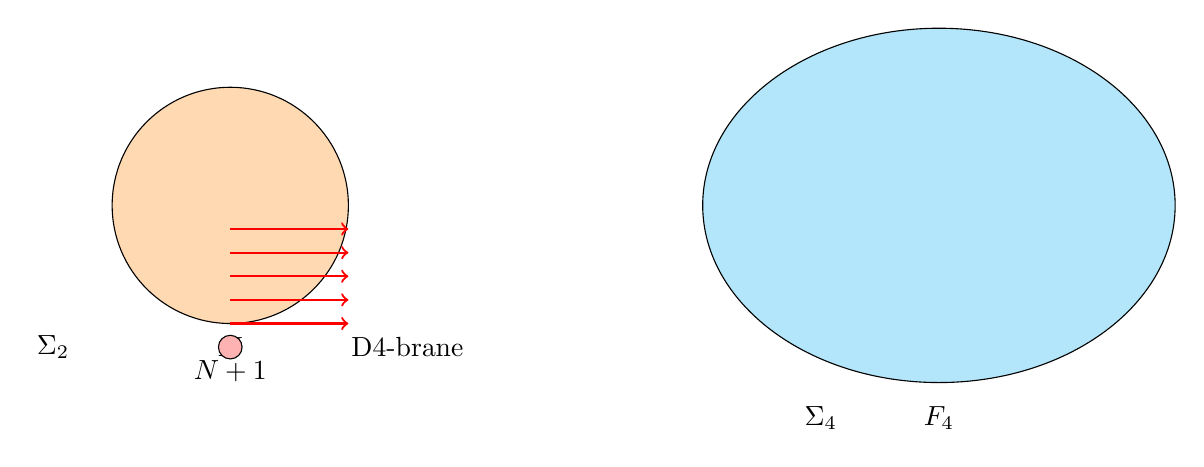
\begin{tikzpicture}[scale=1.5]

% Draw the left circle (D4-brane)
\draw[fill=orange!30] (0,0) circle (1);
\node at (0,-1.2) {$N$};
\node at (-1.5,-1.2) {$\Sigma_{2}$};
\node at (1.5,-1.2) {D4-brane};

% Draw the right circle (F4)
\draw[fill=cyan!30] (6,0) ellipse (2 and 1.5);
\node at (6,-1.8) {$F_{4}$};
\node at (5,-1.8) {$\Sigma_{4}$};

% Draw the D4-brane line
\draw[thick, red, ->] (0,-1) -- (1,-1);
\draw[thick, red, ->] (0,-0.8) -- (1,-0.8);
\draw[thick, red, ->] (0,-0.6) -- (1,-0.6);
\draw[thick, red, ->] (0,-0.4) -- (1,-0.4);
\draw[thick, red, ->] (0,-0.2) -- (1,-0.2);

% Draw the N+1 label
\draw[fill=red!30] (0,-1.2) circle (0.1);
\node at (0,-1.4) {$N+1$};

\end{tikzpicture}

\end{document}